\chapter[MOSFET]{Metal-Oxide-Semiconductor \\ Field-Effect Transistor}

本章使用的符号如表 \ref{tab:mosfet-symbols} 所示。

\begin{table}[!htb]
    \centering
    \caption{MOSFET 符号表}
    \label{tab:mosfet-symbols}
    \begin{NiceTabular}{cccc}
        \Xhline{1pt}
        \textbf{Symbol} & \textbf{Meaning} & \textbf{Unit} & \textbf{Polarity} \\ \hline
        $V_{\rm{TH}}$ & 阈值电压(Threshold voltage) & $\unit{\volt}$ & n$+$, p$-$ \\
        $V_{\rm{DS}}$ & 漏源电压(Drain-source voltage) & $\unit{\volt}$ & n$+$, p$-$ \\
        $V_{\rm{GS}}$ & 栅源电压(Gate-source voltage) & $\unit{\volt}$ & n$+$, p$-$ \\
        $I_{\rm{D}}$ & 漏电流(Drain current) & $\unit{\ampere}$ & n$+$, p$-$ \\
        $I_{\rm{DS}}$ & 漏源电流(Drain-source current) & $\unit{\ampere}$ & n$+$, p$-$ \\
        $W$ & 沟道宽度(Channel width) & $\unit{\meter}$ & $+$ \\
        $L$ & 沟道长度(Channel length) & $\unit{\meter}$ & $+$ \\
        $C_{\rm{ox}}$ & 单位面积氧化层电容(Oxide capacitance) & $\unit{\farad \per \meter \squared}$ & $+$ \\
        $\mu_{\rm{n}}$/$\mu_{\rm{p}}$ & 电子/空穴迁移率(mobility) & $\unit{\meter \squared \per \volt \per \second}$ & $+$ \\
        $k_{\rm{n}}$/$k_{\rm{p}}$ & 增益因子(Gain Factor) & $\unit{\ampere \meter \squared \per \volt \squared}$ & n$+$, p$-$ \\
        $k'_{\rm{n}}$/$k'_{\rm{p}}$ & 工艺跨导(Transconductance) & $\unit{\ampere \meter \squared \per \volt \squared}$ & n$+$, p$-$ \\
        $V_{\rm{DSAT}}$ & 速度饱和电压(Velocity saturation voltage) & $\unit{\volt}$ & n$+$, p$-$ \\
        $\lambda$ & 沟道长度调制系数(Channel length modulation coefficient) & $\unit{\volt \tothe{-1}}$ & n$+$, p$-$ \\
        \Xhline{1pt}
    \end{NiceTabular}
\end{table}

\section[MOS]{Metal-Oxide-Semicounductor Capacitor}

\section{Structure of MOSFET}

MOSFET\footnote{本章中的MOSFET均为绝缘栅型,不考虑结型} 分为两类: \textbf{n-channel(n沟道)} 和 \textbf{p-channel(p沟道)}。其导电载流子分别为电子和空穴。
每一类又分为两种: \textbf{depletion(耗尽型)} 和 \textbf{enhancement(增强型)}。耗尽型的 MOSFET 的沟道是一直存在的,而增强型的 MOSFET 的沟道是需要外加电压才能形成的。

表 \ref{tab:mosfet-types} 总结了这四种 MOSFET 的特点。

\begin{table}[!htb]
    \centering
    \caption{MOSFET 的类型}
    \label{tab:mosfet-types}
    \begin{NiceTabular}{c|cccc}
        \Xhline{1pt}
        & \makecell[c]{{\textbf{N-channel}} \\ \textbf{Depletion}} & \makecell[c]{{\textcolor{deep-blue}{\textbf{N-channel}}} \\ \textcolor{deep-blue}{\textbf{Enhancement}}} & \makecell[c]{{\textbf{P-channel}} \\ \textbf{Depletion}} & \makecell[c]{{\textcolor{deep-red}{\textbf{P-channel}}} \\ \textcolor{deep-red}{\textbf{Enhancement}}} \\ 
        \hline
        \multirowcell{-3}{\textbf{Symbol}} & \includegraphics*[width=0.08\textwidth]{n_dep.pdf} & \includegraphics*[width=0.08\textwidth]{n_enh.pdf} & \includegraphics*[width=0.08\textwidth]{p_dep.pdf} & \includegraphics*[width=0.08\textwidth]{p_enh.pdf} \\
        \multirowcell{-3}{\textbf{Symbol} \\ (arrow)} & \includegraphics*[width=0.08\textwidth]{n_dep_arrow.pdf} & \includegraphics*[width=0.08\textwidth]{n_enh_arrow.pdf} & \includegraphics*[width=0.08\textwidth]{p_dep_arrow.pdf} & \includegraphics*[width=0.08\textwidth]{p_enh_arrow.pdf} \\
        \hline
        \textbf{Oxide} & positive ion doping & no ion doping & negative ion doping & no ion doping \\
        \textbf{Operation} & always on & off when $V_{\rm{GS}} = 0$ & always on & off when $V_{\rm{GS}} = 0$ \\
        \textbf{Source} & n+, electron out & n+, electron out & p+, hole out & p+, hole out \\
        \textbf{Drain} & n+, electron in & n+, electron in & p+, hole in & p+, hole in \\
        \textbf{Gate} & usually VDD & usually VDD & usually GND & usually GND \\
        \textbf{Body/Bulk} & p, usually GND & p, usually GND & n, usually VDD & n, usually VDD \\
        $\bm{V_{\rm{TH}}}$ & negative & positive & positive & negative \\
        $\bm{I_{\rm{D}}}$ & positive & positive & negative & negative \\
        $\bm{V_{\rm{DS}}}$ & positive & positive & negative & negative \\
        $\bm{V_{\rm{GS}}}$ & > $V_{\rm{TH}}$ & > $V_{\rm{TH}}$ & < $V_{\rm{TH}}$ & < $V_{\rm{TH}}$ \\
        \multirowcell{-3}{\textbf{Output} \\ \textbf{Characteristics}} & \includegraphics*[width=0.17\textwidth]{n_dep_out.pdf} & \includegraphics*[width=0.17\textwidth]{n_enh_out.pdf} & \includegraphics*[width=0.17\textwidth]{p_dep_out.pdf} & \includegraphics*[width=0.17\textwidth]{p_enh_out.pdf} \\
        \multirowcell{-3}{\textbf{Transfer} \\ \textbf{Characteristics}} & \includegraphics*[width=0.17\textwidth]{n_dep_tran.pdf} & \includegraphics*[width=0.17\textwidth]{n_enh_tran.pdf} & \includegraphics*[width=0.17\textwidth]{p_dep_tran.pdf} & \includegraphics*[width=0.17\textwidth]{p_enh_tran.pdf} \\
        \Xhline{1pt}
    \end{NiceTabular}
\end{table}

在集成电路设计中,我们通常使用\textbf{增强型 MOSFET},因为它的沟道是需要外加电压才能形成的,可以更好地控制其电流。而耗尽型 MOSFET 的沟道是一直存在的,所以它的电流难以控制。在不作特殊说明的情况下,本章中的 MOSFET 均为增强型。

一个 MOSFET 的结构如图 \ref{fig:mosfet_3d} 所示。

\begin{figure}[!htb]
    \centering
    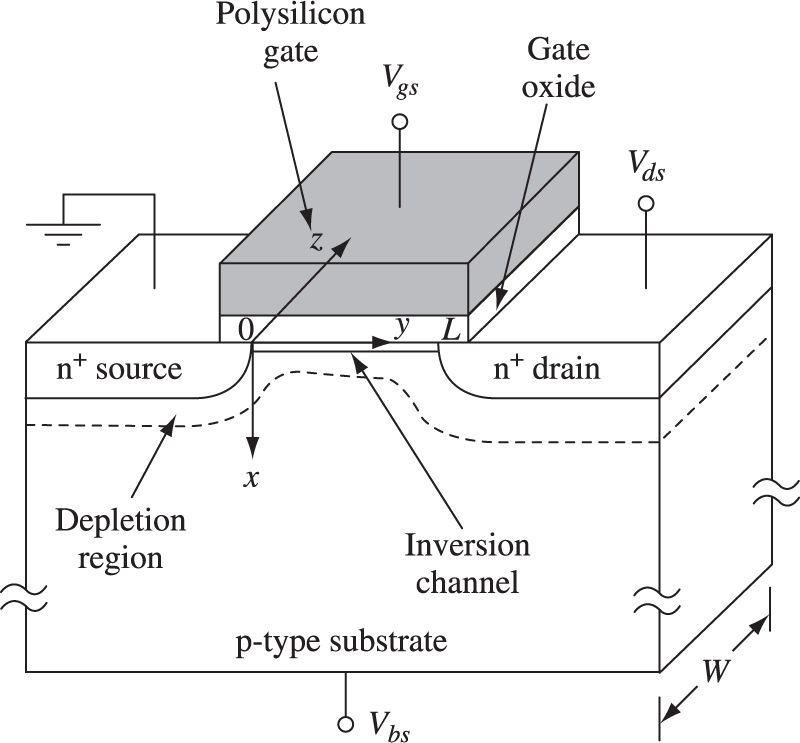
\includegraphics[width=0.5\textwidth]{mosfet_3d.jpg}
    \caption{MOSFET 结构}
    \label{fig:mosfet_3d}
\end{figure}

%%%
\section{Long-Channel MOSFET I-V Characteristics}

MOSFET 有线性(linear)、饱和(saturation)和截止(cutoff)三种工作状态。以 n-channel 为例,其三种工作状态如图 \ref{fig:mosfet_state} 所示。

\begin{figure}[!htb]
    \centering
    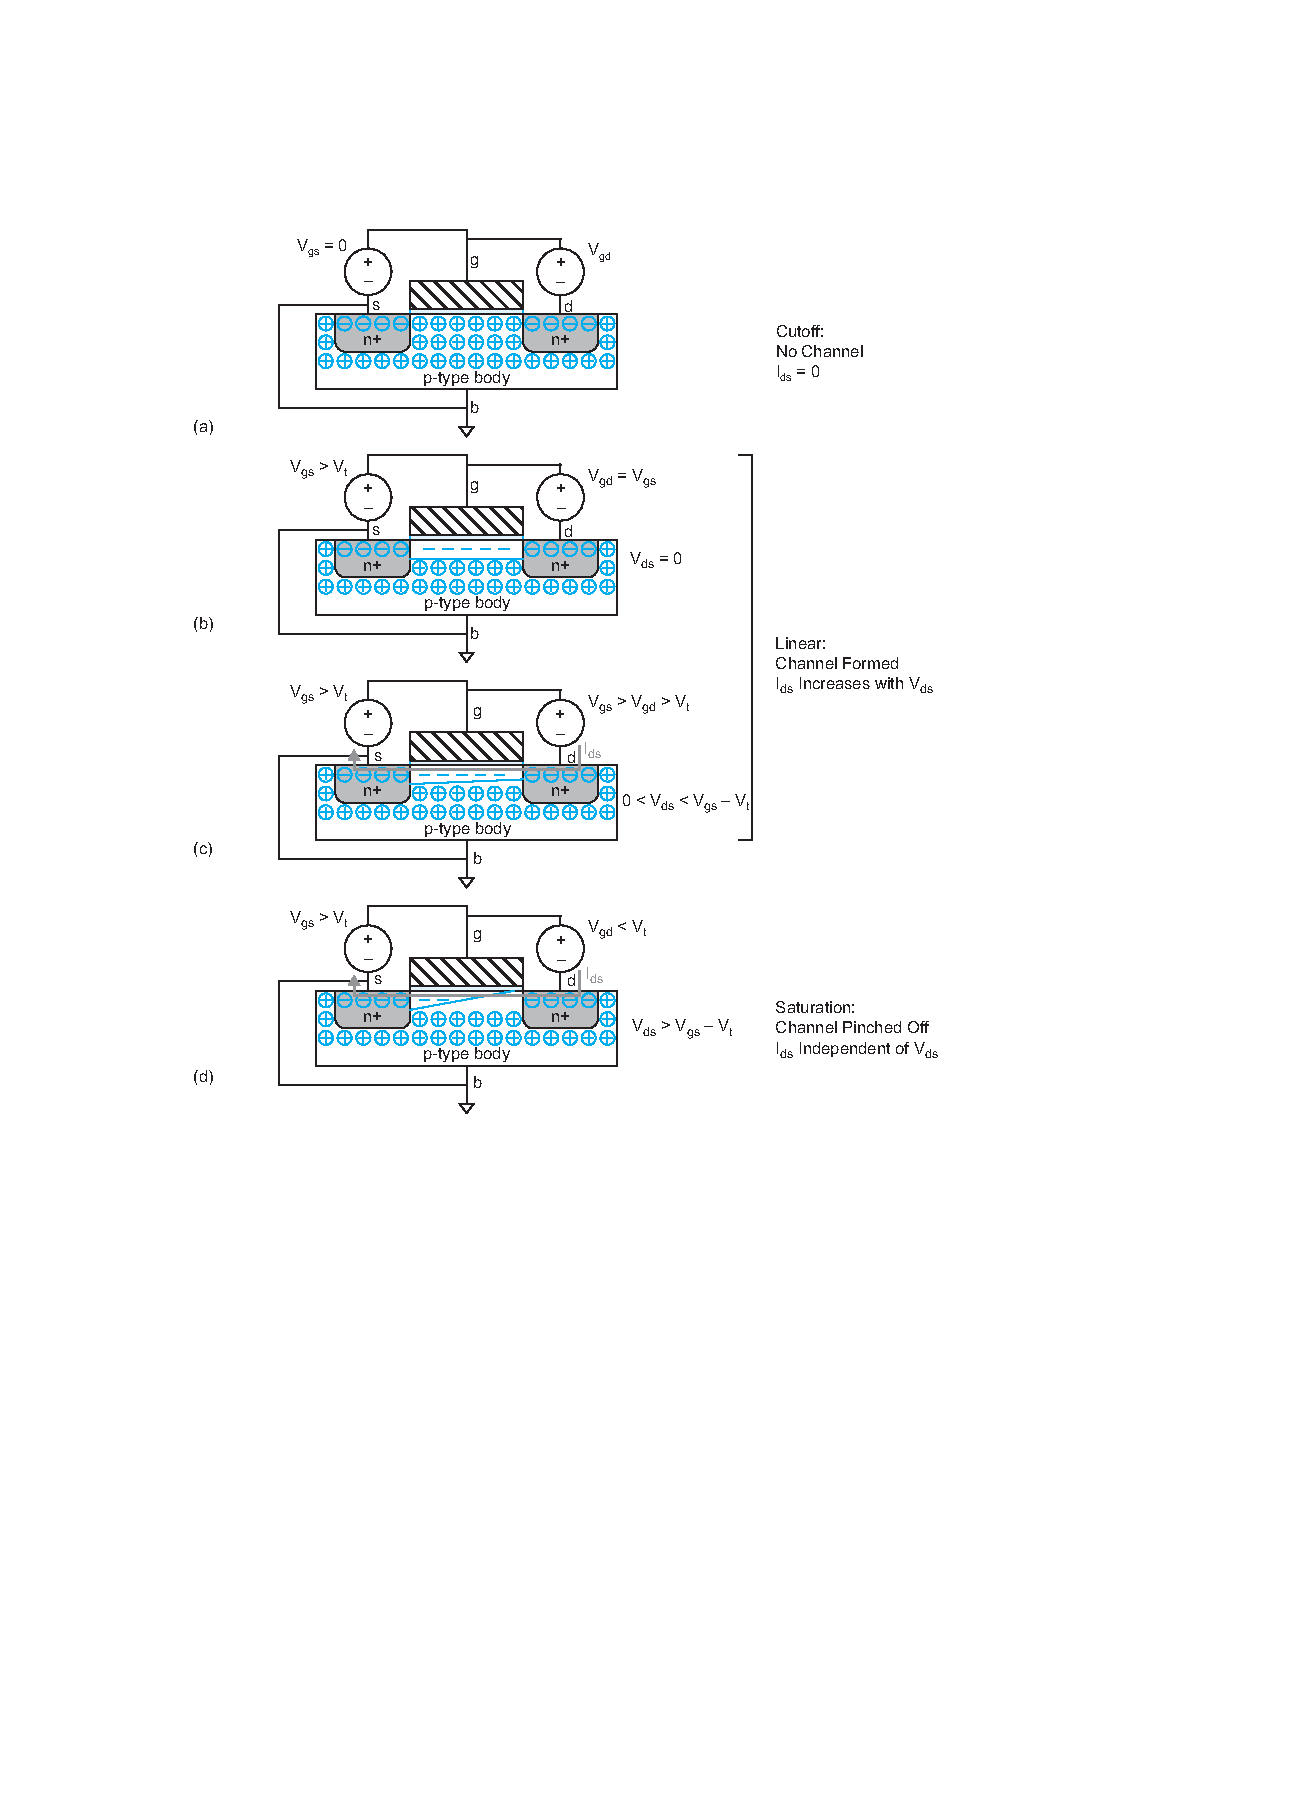
\includegraphics[width=0.7\textwidth]{mosfet_state.pdf}
    \caption{MOSFET 的三种工作状态\cite{CMOS-VLSI}}
    \label{fig:mosfet_state}
\end{figure}

对于 NMOSFET,其 I-V 特性为
\begin{equation}
    I_{\rm{D}} = 
    \begin{dcases}  % 自动调整上下两行的高度, dfrac fix
        \begin{aligned}
            & 0 && V_{\rm{GS}} < V_{\rm{TH}} &&& \text{Cut-off} \\
            & \mu_{\rm{n}} C_{\rm{ox}} \frac{W}{L} \left[ (V_{\rm{GS}} - V_{\rm{TH}}) V_{\rm{DS}} - \frac{V_{\rm{DS}}^2}{2} \right] && V_{\rm{GS}} \geqslant V_{\rm{TH}}, V_{\rm{DS}} \leqslant V_{\rm{GS}} - V_{\rm{TH}} &&& \text{Linear} \\
            & \frac{1}{2} \mu_{\rm{n}} C_{\rm{ox}} \frac{W}{L} (V_{\rm{GS}} - V_{\rm{TH}})^2 && V_{\rm{GS}} \geqslant V_{\rm{TH}}, V_{\rm{DS}} > V_{\rm{GS}} - V_{\rm{TH}} &&& \text{Saturation}
        \end{aligned}
    \end{dcases}
\end{equation}
对于 PMOSFET,其 I-V 特性为
\begin{equation}
    I_{\rm{D}} = 
    \begin{dcases}  % 自动调整上下两行的高度, dfrac fix
        \begin{aligned}
            & 0 && V_{\rm{GS}} > V_{\rm{TH}} &&& \text{Cut-off} \\
            & \mu_{\rm{p}} C_{\rm{ox}} \frac{W}{L} \left[ (V_{\rm{GS}} - V_{\rm{TH}}) V_{\rm{DS}} - \frac{V_{\rm{DS}}^2}{2} \right] && V_{\rm{GS}} \leqslant V_{\rm{TH}}, V_{\rm{DS}} \geqslant V_{\rm{GS}} - V_{\rm{TH}} &&& \text{Linear} \\
            & \frac{1}{2} \mu_{\rm{p}} C_{\rm{ox}} \frac{W}{L} (V_{\rm{GS}} - V_{\rm{TH}})^2 && V_{\rm{GS}} \leqslant V_{\rm{TH}}, V_{\rm{DS}} < V_{\rm{GS}} - V_{\rm{TH}} &&& \text{Saturation}
        \end{aligned}
    \end{dcases}
\end{equation}

%%%
\section{Nonideal I-V Effects}

%%%%
\subsection{Mobility Degradation and Velocity Saturation}

沟道较短的晶体管,也称为短沟器件的行为与长沟器件有所不同,它们不再发生夹断饱和(Pinch-Off Saturation),取而代之的是\textbf{速度饱和(Velocity Saturation)}。

若同时考虑\textbf{速度饱和(Velocity Saturation)}效应,对于 NMOSFET,其 I-V 特性为
\begin{equation}
    I_{\rm{D}} = 
    \begin{dcases}  % 自动调整上下两行的高度, dfrac fix
        \begin{aligned}
            & 0 && \text{Cut-off} \\
            & \mu_{\rm{n}} C_{\rm{ox}} \frac{W}{L} \left[ (V_{\rm{GS}} - V_{\rm{TH}}) V_{\rm{DS}} - \frac{V_{\rm{DS}}^2}{2} \right] && \text{Linear} \\
            & \frac{1}{2} \mu_{\rm{n}} C_{\rm{ox}} \frac{W}{L} (V_{\rm{GS}} - V_{\rm{TH}})^2 && \text{Saturation} \\
            & \mu_{\rm{n}} C_{\rm{ox}} \frac{W}{L} \left[ (V_{\rm{GS}} - V_{\rm{TH}}) V_{\rm{DSAT}} - \frac{V_{\rm{DSAT}}^2}{2} \right] && \text{Velocity Saturation}
        \end{aligned}
    \end{dcases}
\end{equation}
各个状态的电压关系为
\begin{equation}
    \begin{aligned}
        & \text{Cut-off:} && V_{\rm{GS}} < V_{\rm{TH}} \\
        & \text{Linear:} && V_{\rm{GS}} \geqslant V_{\rm{TH}}, \min \left(V_{\rm{GS}} - V_{\rm{TH}}, V_{\rm{DS}}, V_{\rm{DSAT}}\right) = V_{\rm{DS}} \\
        & \text{Saturation:} && V_{\rm{GS}} \geqslant V_{\rm{TH}}, \min \left(V_{\rm{GS}} - V_{\rm{TH}}, V_{\rm{DS}}, V_{\rm{DSAT}}\right) = V_{\rm{GS}} - V_{\rm{TH}} \\
        & \text{Velocity Saturation:} && V_{\rm{GS}} \geqslant V_{\rm{TH}}, \min \left(V_{\rm{GS}} - V_{\rm{TH}}, V_{\rm{DS}}, V_{\rm{DSAT}}\right) = V_{\rm{DSAT}}
    \end{aligned}
\end{equation}
而对于 PMOSFET,其 I-V 特性公式与 NMOSFET 相同,但得到的 $I_{\rm{D}}$ 为负值。
\begin{equation}
    I_{\rm{D}} = 
    \begin{dcases}  % 自动调整上下两行的高度, dfrac fix
        \begin{aligned}
            & 0 && \text{Cut-off} \\
            & -\mu_{\rm{p}} C_{\rm{ox}} \frac{W}{L} \left[ (V_{\rm{GS}} - V_{\rm{TH}}) V_{\rm{DS}} - \frac{V_{\rm{DS}}^2}{2} \right] && \text{Linear} \\
            & -\frac{1}{2} \mu_{\rm{p}} C_{\rm{ox}} \frac{W}{L} (V_{\rm{GS}} - V_{\rm{TH}})^2 && \text{Saturation} \\
            & -\mu_{\rm{p}} C_{\rm{ox}} \frac{W}{L} \left[ (V_{\rm{GS}} - V_{\rm{TH}}) V_{\rm{DSAT}} - \frac{V_{\rm{DSAT}}^2}{2} \right] && \text{Velocity Saturation}
        \end{aligned}
    \end{dcases}
\end{equation}
各个状态的电压关系为
\begin{equation}
    \begin{aligned}
        & \text{Cut-off:} && V_{\rm{GS}} > V_{\rm{TH}} \\
        & \text{Linear:} && V_{\rm{GS}} \leqslant V_{\rm{TH}}, \max \left(V_{\rm{GS}} - V_{\rm{TH}}, V_{\rm{DS}}, V_{\rm{DSAT}}\right) = V_{\rm{DS}} \\
        & \text{Saturation:} && V_{\rm{GS}} \leqslant V_{\rm{TH}}, \max \left(V_{\rm{GS}} - V_{\rm{TH}}, V_{\rm{DS}}, V_{\rm{DSAT}}\right) = V_{\rm{GS}} - V_{\rm{TH}} \\
        & \text{Velocity Saturation:} && V_{\rm{GS}} \leqslant V_{\rm{TH}}, \max \left(V_{\rm{GS}} - V_{\rm{TH}}, V_{\rm{DS}}, V_{\rm{DSAT}}\right) = V_{\rm{DSAT}}
    \end{aligned}
\end{equation}

%%%%
\subsection{Channel Length Modulation}
沟道长度调制(Channel Length Modulation)是指沟道长度的变化会导致沟道电阻的变化,从而影响沟道电流。当栅和漏之间的电压差增大时,实际的反型沟道长度逐渐减小。
假设$\Delta L / L$与$V_{\rm{DS}}$为线性关系,满足
\begin{equation}
    \frac{\Delta L}{L} = \lambda V_{\rm{DS}}
\end{equation}
其中 $\lambda$ 即为沟道长度调制系数。在饱和区,电流值需要乘上修正系数 $\left(1 + \lambda V_{\rm{DS}}\right)$,即
\begin{equation}
    I_{\rm{D}} = \frac{1}{2} \mu_{\rm{n}} C_{\rm{ox}} \frac{W}{L} \left( V_{\rm{GS}} - V_{\rm{TH}} \right)^2 \eqnmark[RoyalPurple]{lb}{\left( 1 + \lambda V_{\rm{DS}} \right)}
\end{equation}
需要注意,沟道长度调制仅在饱和区生效,只有在饱和区才会出现沟道长度的变化$\Delta L$。

%%%%
\subsection{Subthreshold Conduction}

%%%
\subsection{Threshold Voltage Effects}
\subsubsection{Body Effect}

\subsubsection{Drain-Induced Barrier Lowering}

\subsubsection{Short Channel Effect}

%%%
\section{MOSFET I-V Characteristics Summary}

为了简化公式,引入工艺因子(Gain Factor)和工艺跨导(Transconductance)的概念。\\
工艺因子 $k$ 为
\begin{equation}
    \begin{aligned}
        k_{\rm{n}} &= \mu_{\rm{n}} C_{\rm{ox}} \frac{W}{L} \\
        k_{\rm{p}} &= -\mu_{\rm{p}} C_{\rm{ox}} \frac{W}{L}
    \end{aligned}
\end{equation}
工艺跨导 $k'$ 为
\begin{equation}
    \begin{aligned}
        k'_{\rm{n}} &= \mu_{\rm{n}} C_{\rm{ox}} \\
        k'_{\rm{p}} &= -\mu_{\rm{p}} C_{\rm{ox}}
    \end{aligned}
\end{equation}

这样,NMOSFET 的 I-V 特性为(非截止区)
\begin{equation}
    I_{\rm{D}} = k_{\rm{n}} \left[ (V_{\rm{GS}} - V_{\rm{TH}}) V_{\rm{min}} - \frac{V_{\rm{min}}^2}{2} \right] \left(1 + \lambda V_{\rm{DS}}\right)
\end{equation}
其中 $V_{\rm{min}} = \min \left(V_{\rm{GS}} - V_{\rm{TH}}, V_{\rm{DS}}, V_{\rm{DSAT}}\right)$。\\
PMOSFET 的 I-V 特性为
\begin{equation}
    I_{\rm{D}} = k_{\rm{p}} \left[ (V_{\rm{GS}} - V_{\rm{TH}}) V_{\rm{max}} - \frac{V_{\rm{max}}^2}{2} \right] \left(1 + \lambda V_{\rm{DS}}\right)
\end{equation}
其中 $V_{\rm{max}} = \max \left(V_{\rm{GS}} - V_{\rm{TH}}, V_{\rm{DS}}, V_{\rm{DSAT}}\right)$。

\begin{figure}
    \centering
    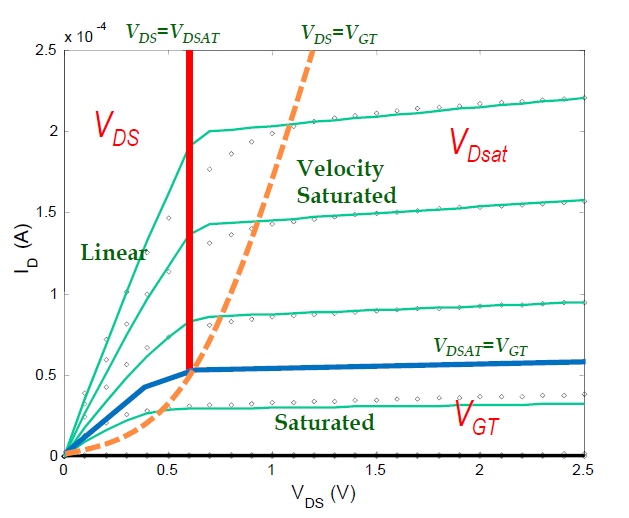
\includegraphics[width=0.5\textwidth]{nmos_iv_regions.png}
    \caption{NMOSFET 的 工作状态}
    \label{fig:nmos_iv_regions}
\end{figure}

%%%
\section{MOSFET C-V Characteristics}
